% !TeX document-id = {7b7d88a4-0972-4202-9c89-33327d1050f5}
% !TeX spellcheck = en_EN
\documentclass[10pt, dvipsnames]{beamer}
\usepackage{appendixnumberbeamer}
\usepackage[T1]{fontenc}
\usepackage[utf8]{inputenc}
\usepackage{hyperref}
\usepackage{fontawesome5, lipsum}
\usepackage{graphicx}
\usepackage[ngerman]{babel}
\usepackage{setspace, multicol, makecell, booktabs, multirow}
\usepackage{mathtools, amsthm, amsfonts, siunitx, physics, chemformula, empheq}
\usepackage{mtpro2, pifont, custom}
\pdfmapfile{=mtpro2.map}
\usepackage[backend=biber, abbreviate=true, doi=false, style=numeric-comp, giveninits=true, sorting=none]{biblatex}
\usepackage{enumitem, csquotes, xurl}
\usepackage[most]{tcolorbox}
\usepackage{multimedia, tikz, tikz-3dplot, pgfplots}
\usepackage[font=footnotesize, bf, format=plain, font=normalsize]{caption}

\usetikzlibrary{math, arrows.meta, calc, angles, quotes, arrows, shapes.geometric, decorations.pathmorphing, overlay-beamer-styles, patterns.meta}

\tikzset{
	partial ellipse/.style args={#1:#2:#3}{
		insert path={+ (#1:#3) arc (#1:#2:#3)}
	}
}

\tikzset{snake arrow/.style=
	{-Latex,
		decorate,
		decoration={snake,amplitude=.4mm,segment length=2mm,post length=1mm}},
}

\graphicspath{ {./bilder/} }
\addbibresource{Literatur.bib}

%\catcode`_=\active
%\newcommand_[1]{\ensuremath{\sb{\fontfamily{Times New Roman}\selectfont \mathrm{#1}}}}

\AtBeginDocument{\sisetup{per-mode = symbol, sticky-per, mode=text, text-font-command=\fontfamily{Times New Roman}\selectfont}}
\let\oldunit\unit
\renewcommand{\unit}[1]{\hspace{4pt}\oldunit{#1}}
\DeclareSIUnit\year{yr}
\DeclareSIUnit\FU{F.U.}

\newcommand{\nair}{n\sb{\fontfamily{Times New Roman}\selectfont \mathrm{air}}}

\usepackage{scalerel,stackengine}
\newcommand\equalhat{\mathrel{\stackon[1.5pt]{=}{\stretchto{%
				\scalerel*[\widthof{=}]{\wedge}{\rule{1ex}{3ex}}}{0.5ex}}}}

% ------------------------------------------------------------------------------
% Use the beautiful metropolis beamer template
% ------------------------------------------------------------------------------
%\usepackage{FiraSans} 
\mode<presentation>
{
	\usetheme[progressbar=frametitle,background=light]{metropolis} 
	\usecolortheme{default} % or try albatross, beaver, crane, ...
	\usefonttheme[onlymath]{serif}  % or try serif, structurebold, ...
	\setbeamertemplate{navigation symbols}{}
	\setbeamertemplate{caption}[numbered]
	\setbeamertemplate{section in toc}[sections numbered]
	\setbeamerfont{frametitle}{size=\LARGE}
	\metroset{block=fill}
} 

\makeatletter
\setlength{\metropolis@progressinheadfoot@linewidth}{3pt}
\setlength{\metropolis@titleseparator@linewidth}{3pt}
\setlength{\metropolis@progressonsectionpage@linewidth}{3pt}

\makeatother

% ------------------------------------------------------------------------------
% tcolorbox / tcblisting
% ------------------------------------------------------------------------------	
\definecolor{MyBlue}{HTML}{0072B2}
\definecolor{MyOrange}{HTML}{D55E00}
\definecolor{MyRed}{HTML}{F00F0F}
\definecolor{MyGreen}{HTML}{20B312}
\definecolor{bg}{HTML}{FBFBFB}

\newcommand{\s}[1]{{\color{MyBlue}#1}}

\setstretch{1.5}

\newtcolorbox{quotebox}{enhanced, colframe=MyOrange, top=0.2cm, bottom=0.2cm, colback=orange!15, left=0.1cm}

\title{relativistische Betrachtung von Bewegungen}
\author{Alexander Helbok}
\date{\today}

\begin{document}
	\maketitle

	\begin{frame}{Radiobeobachtungen}
		\centering
		\vspace*{0.4cm}
		\begin{columns}
			\begin{column}{.5\textwidth}
				\centering
				\begin{tikzpicture}
					\node[anchor=south west,inner sep=0] (image) at (0,0) {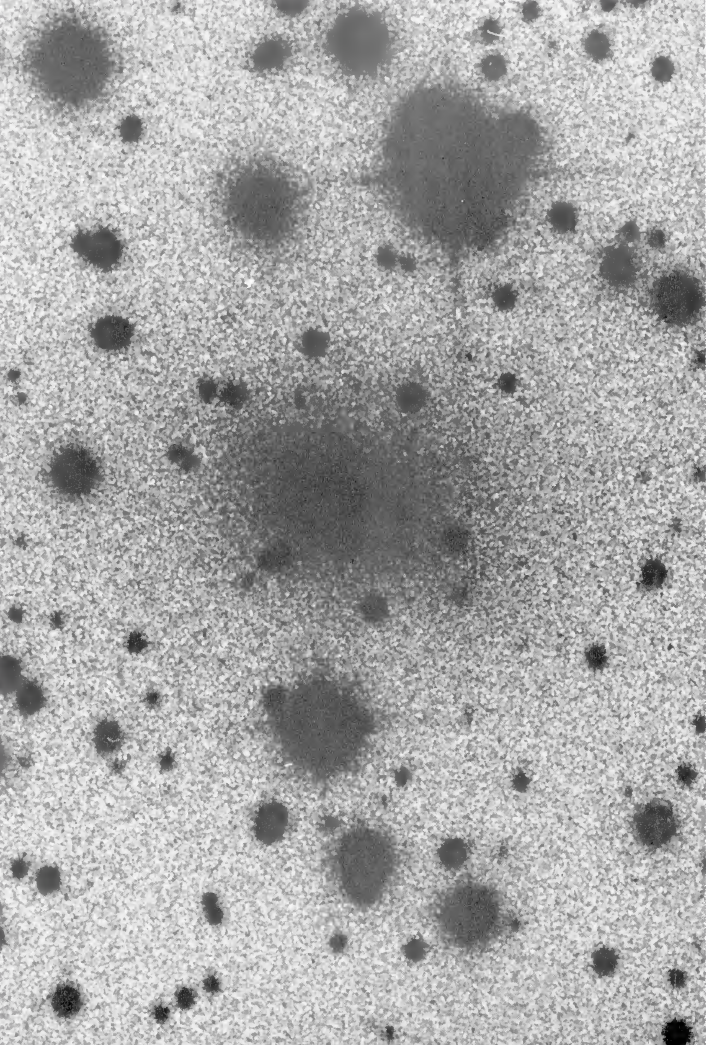
\includegraphics[scale=0.26]{radio1}};
					
					\begin{scope}[x={(image.south east)},y={(image.north west)}]
						\node[] at (0.35, -0.02) {\tiny(\citeauthor{radio} \citeyear{radio})};
					\end{scope}
				\end{tikzpicture}
			\end{column}
			\begin{column}{.5\textwidth}
				\centering
				\begin{tikzpicture}
					\node[anchor=south west,inner sep=0] (image) at (0,0) {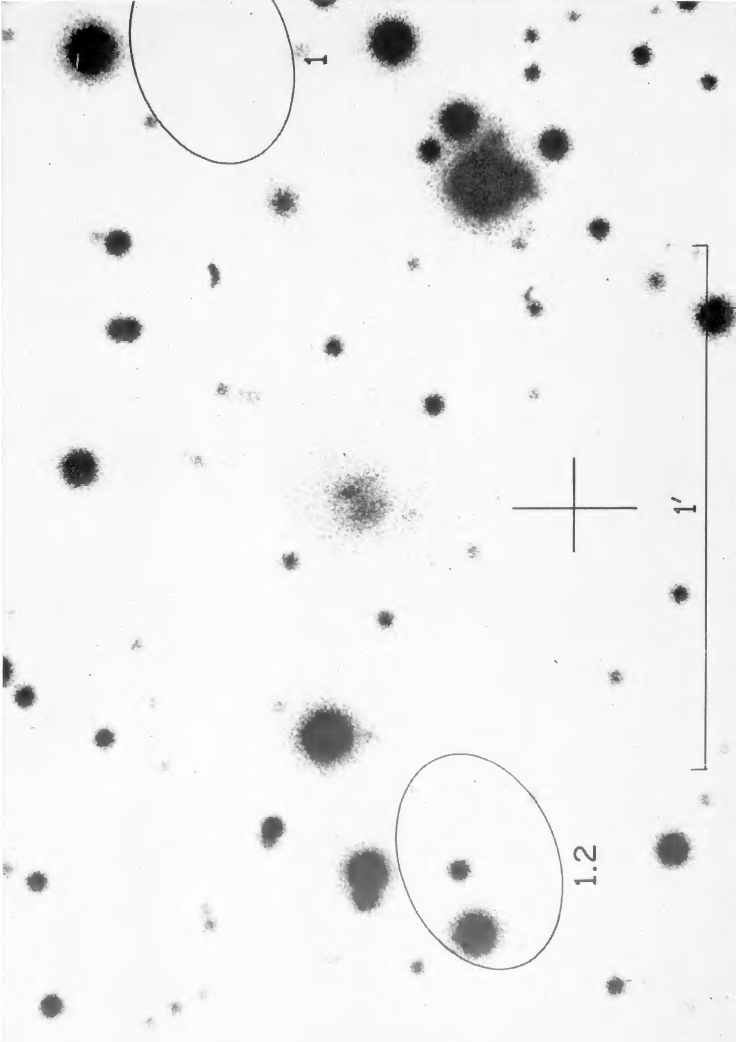
\includegraphics[scale=0.26]{radio2}};
					
					\begin{scope}[x={(image.south east)},y={(image.north west)}]
						\node[] at (0.35, -0.02) {\tiny(\citeauthor{radio} \citeyear{radio})};
					\end{scope}
				\end{tikzpicture}
			\end{column}
		\end{columns}
	\end{frame}
	
	\begin{frame}{Leuchtkraft von 3C 273}
		%Axis Angles
		\tdplotsetmaincoords{70}{90}
		%Macros
		\pgfmathsetmacro{\rvec}{6}
		\pgfmathsetmacro{\thetavec}{65}
		\pgfmathsetmacro{\phivec}{55}
		
		\pgfmathsetmacro{\dphivec}{30}
		\pgfmathsetmacro{\dthetavec}{20}
		%Layers
		\pgfdeclarelayer{background}
		
		\pgfsetlayers{background, main}
		\begin{columns}
			\begin{column}{0.6\textwidth}
				\vspace{-1cm}
				\begin{tikzpicture}[tdplot_main_coords, scale=0.65]
					%Coordinates
					\coordinate (O) at (0,0,0);
					%
					\tdplotsetcoord{A}{\rvec}{\thetavec}{\phivec}
					\tdplotsetcoord{B}{\rvec}{\thetavec + \dthetavec}{\phivec}
					\tdplotsetcoord{C}{\rvec}{\thetavec + \dthetavec}{\phivec + \dphivec}
					\tdplotsetcoord{D}{\rvec}{\thetavec}{\phivec + \dphivec}
					%
					\tdplotsetcoord{A'}{\rvec + 4}{\thetavec}{\phivec}
					\tdplotsetcoord{B'}{\rvec + 3}{\thetavec + \dthetavec}{\phivec}
					\tdplotsetcoord{C'}{\rvec + 1}{\thetavec + \dthetavec}{\phivec + \dphivec}
					\tdplotsetcoord{D'}{\rvec + 2}{\thetavec}{\phivec + \dphivec}
					%		
					%Help Lines
					\begin{pgfonlayer}{background}
						%Up
						\draw[] (O) -- (A') node [pos=0, below] {\( L \)};
						\draw (O) -- (B') node[pos=0.4, below] {$d$};
						\draw (O) -- (C') node [pos=0.9, above, yshift=0] {\( F \)};
						\draw[] (O) -- (D');
					\end{pgfonlayer}
					
					\begin{scope}
						%Fill Color
						\begin{pgfonlayer}{main}
							\clip[canvas is zy plane at x=0] (\rvec - 0.09,0) arc (0:200:\rvec - 0.09);
							%Front
							\filldraw[opacity=0.6, color=black, fill=MyOrange, thick] (A) to[bend left=4] (B)  to[bend left=2] (C) to[bend right=6.5] (D) to[bend right=4] cycle;
						\end{pgfonlayer}
						
						\draw[canvas is zy plane at x=0, ultra thick, MyBlue] (\rvec - 0.1,0) arc (0:200:\rvec - 0.1);	
					\end{scope}
				\end{tikzpicture}
			\end{column}
			\begin{column}{0.45\textwidth}
				\centering
				\begin{tikzpicture}
					\draw[-latex, shorten >=0.35cm] (0.5, -1) -- (0.8, 0);
					\node at (0, -1) [below, align=center] {Flussmessung im Radiobereich};
					
					\node at (0, 0) {\( L = 4\pi d^2F \)};
					
					\draw[-latex, shorten >=0.35cm] (0, 1) -- (0.4, 0);
					\node [align=center, above] at (0, 1) {Entfernung über Rotverschiebung\\ (\( z = 0.158 \))};
					
					\node [] at (0, -3) {\( \Rightarrow \) extrem Hell};
				\end{tikzpicture}
			\end{column}
		\end{columns}
	\end{frame}
	
	\begin{frame}{Helligkeitsschwankungen in 3C 273}
		\begin{columns}
			\begin{column}{0.5\textwidth}
				\vspace{-0.35cm}
				\begin{tikzpicture}
					\node[anchor=south west,inner sep=0] (image) at (0,0) {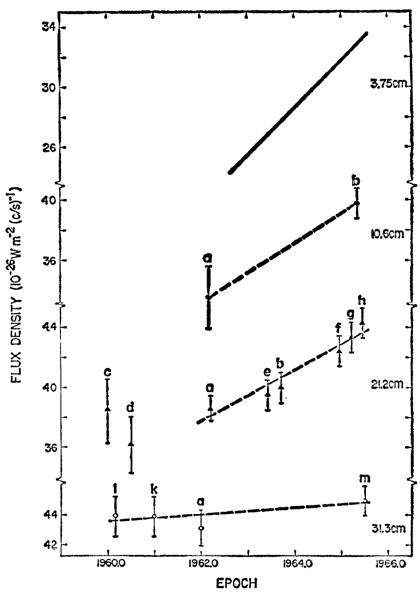
\includegraphics[scale=0.33]{oldflux-}};
					
					\begin{scope}[x={(image.south east)},y={(image.north west)}]
						\node[] at (0.4, 0.925) {\tiny(\citeauthor{oldflux} \citeyear{oldflux})};
					\end{scope}
				\end{tikzpicture}
			\end{column}
			\begin{column}{0.5\textwidth}
				\hspace{-0.3cm}\vspace{-0.25cm}
				\begin{tikzpicture}
					\node[anchor=south west,inner sep=0] (image) at (0,0) {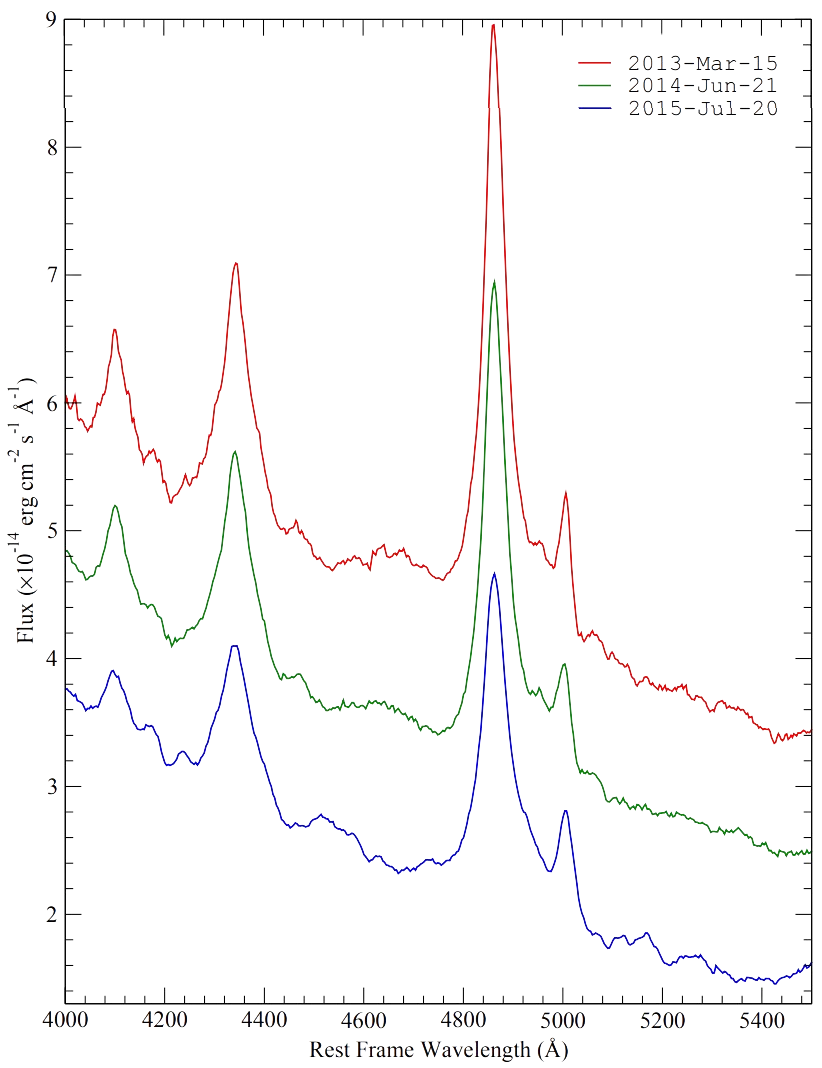
\includegraphics[scale=0.185]{newflux}};
					
					\begin{scope}[x={(image.south east)},y={(image.north west)}]
						\node[align=left] at (0.3, 0.925) {\tiny(\citeauthor{newflux} \citeyear{newflux})};
					\end{scope}
				\end{tikzpicture}
			\end{column}
		\end{columns}
	\end{frame}
	
	\begin{frame}{Fluktuationen erklärt}
		\begin{columns}
			\begin{column}{0.3\textwidth}
				\begin{tikzpicture}		
					\begin{scope}
						\clip[] (-0.5, 2) rectangle (0, 6);
						\fill[pattern={Lines[distance=3mm,angle=45,line width=0.4mm]}] (-1, 1) rectangle (0, 6);
					\end{scope}
					
					\draw[latex-latex] (-0.7,2) -- (-0.7,6) node [above, pos=0.5, rotate=90] {\( 2 \) Lichtjahre};
						
					\foreach \i in {1, 2, 3}{
						\coordinate (P\i) at (0, 2*\i);
						\draw[snake arrow, MyOrange] (P\i) -- (1, 2*\i);}
						
					\uncover<2-4>{\draw[snake arrow, MyRed, thick] (P1) -- (1, 2);}
					\uncover<3-6>{\draw[snake arrow, MyRed, thick] (P2) -- (1, 4);}
					\uncover<4-7>{\draw[snake arrow, MyRed, thick] (P3) -- (1, 6);}
					
					\draw[thick, line cap=round, MyOrange, thick, opacity=1] (P1) -- (P3);
					
					\only<3>{\draw[thick, line cap=round, MyRed, ultra thick, opacity=1] (P1) -- (P2);}
					\only<4-5>{\draw[thick, line cap=round, MyRed, ultra thick, opacity=1] (P1) -- (P3);}
					\only<6>{\draw[thick, line cap=round, MyRed, ultra thick, opacity=1] (P3) -- (P2);}
					
					\only<8>{};
				\end{tikzpicture}
			\end{column}
			\begin{column}{0.7\textwidth}
				\begin{tikzpicture}
					\begin{axis}[
						axis lines = left,
						axis line style = ultra thick,
						xlabel = \(t\) in Jahren,
						ylabel = {Fluss},
						enlargelimits=true,
						xtick={0, 1, 2, 3, 4, 5, 6},
						ytick={1, 2},
						xmin=0,
						xmax=6,
						ymin=1,
						ymax=2,
						tick align=inside,
						tickwidth=5pt,
						yticklabels={\( F_0 \), \( 2F_0 \)}]
					\only<1->{\addplot [domain=-1:0, color=MyBlue, thick] {1};}
					\only<3->{\addplot [domain=0:1, color=MyBlue, thick] {x/2+1};}
					\only<4->{\addplot [domain=1:2, color=MyBlue, thick] {x/2+1};}
					\only<5->{\addplot [domain=2:3, color=MyBlue, thick] {2};}
					\only<6->{\addplot [domain=3:4, color=MyBlue, thick] {-x/2+3.5};}
					\only<7->{\addplot [domain=4:5, color=MyBlue, thick] {-x/2+3.5};}
					\only<8->{\addplot [domain=5:6, color=MyBlue, thick] {1};}
				\end{axis}
			\end{tikzpicture}
			\end{column}
		\end{columns}
	\end{frame}
	
	\begin{frame}{Helligkeitsschwankungen in 3C 273}
		\begin{columns}
			\begin{column}{0.5\textwidth}
				\vspace{-0.35cm}
				\begin{tikzpicture}
					\node[anchor=south west,inner sep=0] (image) at (0,0) {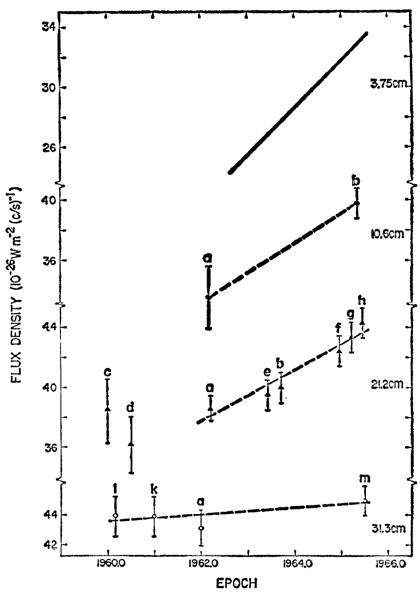
\includegraphics[scale=0.33]{oldflux-}};
					
					\begin{scope}[x={(image.south east)},y={(image.north west)}]
						\node[] at (0.4, 0.925) {\tiny(\citeauthor{oldflux} \citeyear{oldflux})};
					\end{scope}
				\end{tikzpicture}
			\end{column}
			\begin{column}{0.5\textwidth}
				\hspace{-0.3cm}\vspace{-0.25cm}
				\begin{tikzpicture}
					\node[anchor=south west,inner sep=0] (image) at (0,0) {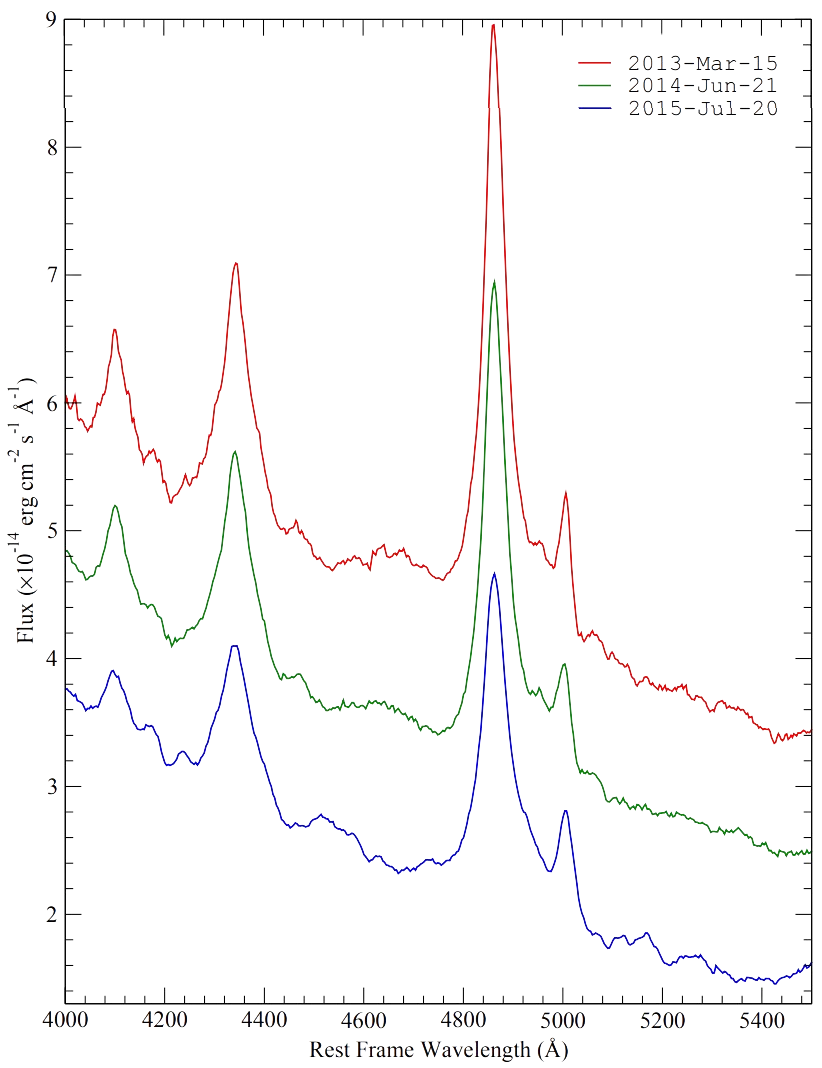
\includegraphics[scale=0.185]{newflux}};
					
					\begin{scope}[x={(image.south east)},y={(image.north west)}]
						\node[align=left] at (0.3, 0.925) {\tiny(\citeauthor{newflux} \citeyear{newflux})};
					\end{scope}
				\end{tikzpicture}
			\end{column}
		\end{columns}
	\end{frame}
	
%	########### Theorie #############
%	\begin{frame}{Winkeldurchmesser}
%		\begin{tikzpicture}[scale=1.4]
%			\coordinate (O) at (6,1.5);
%			\coordinate (S) at (0,1.5);
%			\coordinate (U) at (0,3);
%			
%			\filldraw[ball color=white] (S) circle (1.5);
%			
%			\draw[dashed,color=darkgray] (0,0) arc (-90:90:0.5 and 1.5);% right half of the left ellipse
%			\draw[thick] (0,0) -- (O);% bottom line
%			\draw[thick] (U) -- (O);% top line
%			\draw[thick] (0,0) arc (270:90:0.5 and 1.5);% left half of the left ellipse
%			
%			\draw[fill] (S) circle (0.05) node [below, yshift=-2] {\( S \)};
%			\draw[fill] (O) circle (0.05) node [above, yshift=2] {\( O \)};
%			
%			\draw[semithick, dashed] (O) -- (S) node [above, pos=0.6] {\( R \)};
%			\draw[semithick, dashed] (S) -- (U) node [left, pos=0.5] {\( r \)}; 
%			
%			\pic [draw, angle radius=3cm] {angle = U--O--S};
%			\pic [draw, angle radius=0.25cm, thick] {right angle = O--S--U};
%			
%			\draw (4.5, 1.7) node {\( \theta \)};
%		\end{tikzpicture}	
%		\vspace{-1cm}\hspace{4cm}
%		\begin{minipage}{.5\textwidth}
%			\begin{quotebox}
%				\( r \ll R,\ \tan(\theta) \approx \theta \)\\
%				\( \sphericalangle = 2\theta = 2\tfrac{r}{R} \)
%			\end{quotebox}
%%			
%		\end{minipage}
%	\end{frame}
	
	\begin{frame}{sphärische Expansion \( v \ll c \)}
		\begin{tikzpicture}[every node/.style={scale=0.9}, scale=1.4]
	%		\node[inner sep=0pt] (russell) at (0,0.05){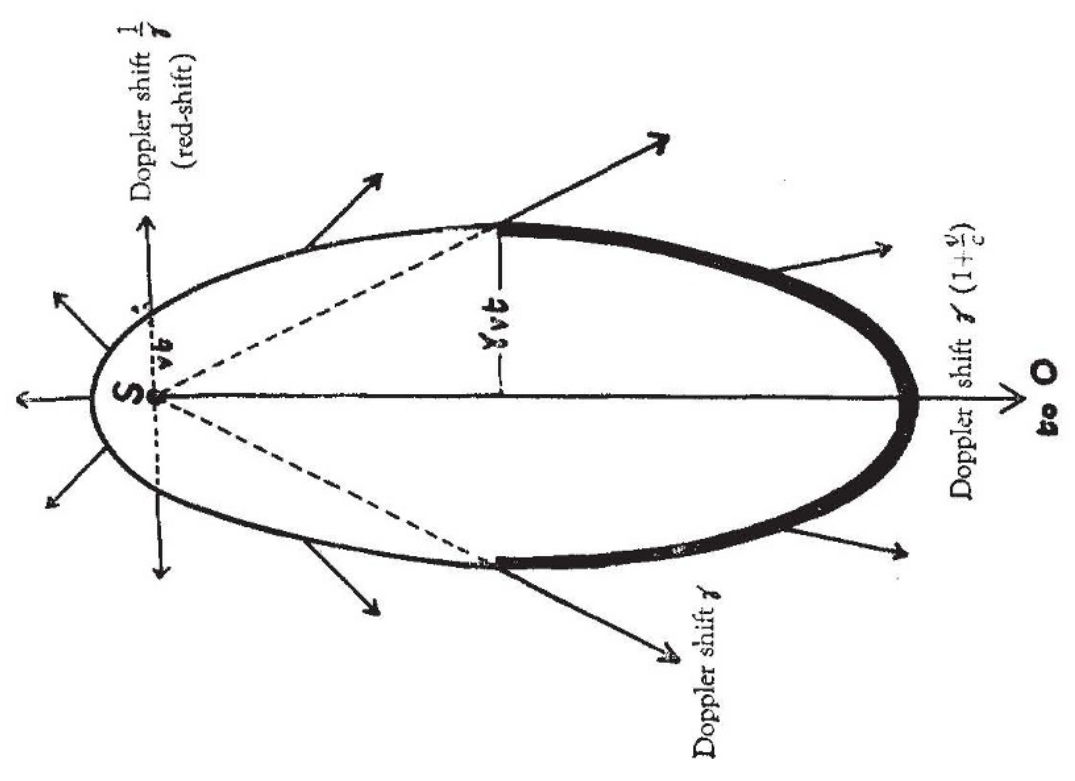
\includegraphics[scale=0.25]{bilder/aberration2}};
	
	%		\draw [step=.1, gray,thin, opacity=0.5] (-4,-2) grid (4,2);
	%		\draw [step=1, black, opacity=0.5] (-4,-2) grid (4,2);
			
			\coordinate (S) at (-2.5, 0);
			
			\draw[-latex] (S) -- (-3.5, 0);
			
			\draw[-latex] (S) -- (-2.5+0.7,  0.7);
			\draw[-latex] (S) -- (-2.5+0.7, -0.7);
			
			\draw[-latex] (S) -- (-2.5-0.7,  0.7);
			\draw[-latex] (S) -- (-2.5-0.7, -0.7);
			
			\draw[-latex] (S) -- (-2.5, 1);
			\draw[-latex] (S) -- (-2.5, -1);
			
			
			\draw[fill=bg] (S) circle (0.6);
			
			\draw[MyBlue, line cap=round, thick] (S) -- (-2.5, 0.6) node [right, pos=0.55] {\( v t \)};
			
			\draw[thick] (S) circle (0.6);
			
			\draw[line width=2.5, MyOrange, opacity=0.75, line cap=round] (-2.5, -0.6) arc (-90:90:0.6);
			
			\draw[fill] (S) circle (0.05cm) node [below, yshift=-1] {\( S \)};
			
			\draw[-latex, semithick] (S) -- (3.5, 0) node [above left, pos=0.975] {to \( O \)};
		\end{tikzpicture}
	\end{frame}
	
	\begin{frame}{sphärische Expansion \( v \sim c \)}
		\begin{tikzpicture}[every node/.style={scale=0.9}, scale=1.4]
	%		\node[inner sep=0pt] (russell) at (0,0.05){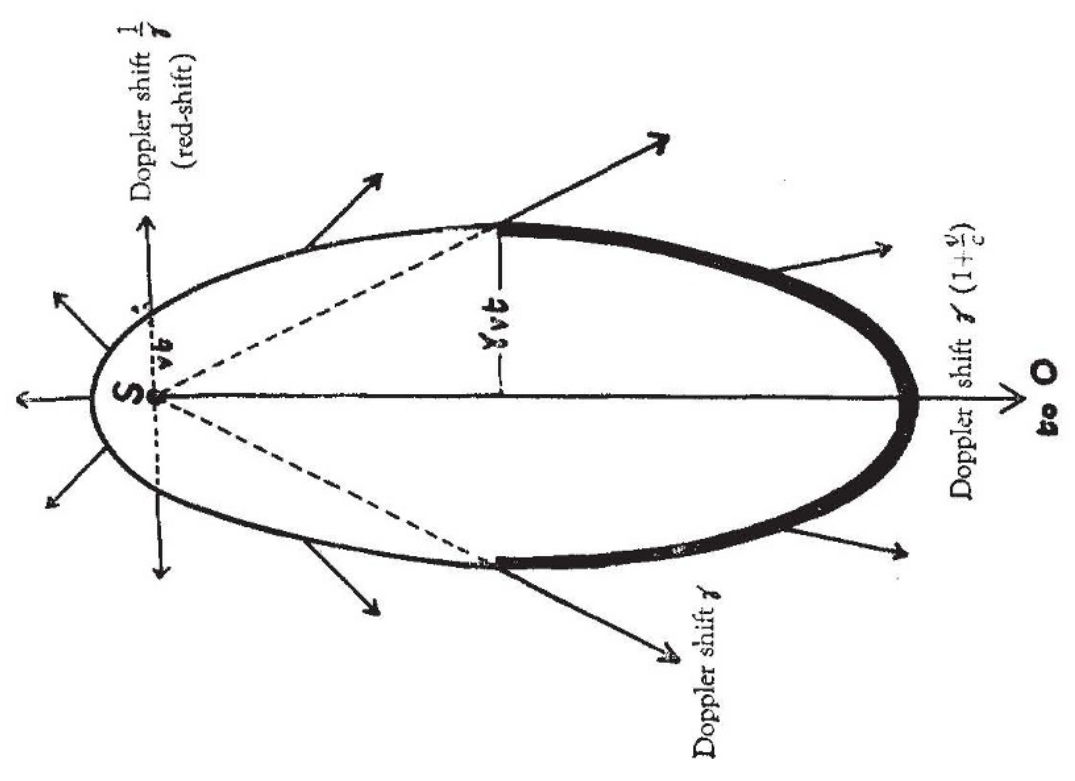
\includegraphics[scale=0.25]{bilder/aberration2}};
	
	%		\draw [step=.1, gray,thin, opacity=0.5] (-4,-2) grid (4,2);
	%		\draw [step=1, black, opacity=0.5] (-4,-2) grid (4,2);
			
			\coordinate (S) at (-2.5, 0);
			
			\draw[-latex] (S) -- (-3.5, 0);
			
			\draw[-latex] (S) -- (-3.2, 0.7);
			\draw[-latex] (S) -- (-3.2, -0.7);
			
			\draw[-latex] (S) -- (-2.5, 1.2);
			\draw[-latex] (S) -- (-2.5, -1.2);
			
			\draw[-latex] (S) -- (-1, 1.5);
			\draw[-latex] (S) -- (-1, -1.5);
			
			\draw[-latex] (S) -- (0.9, 1.7);
			\draw[-latex] (S) -- (0.9, -1.7);
			
			\draw[-latex] (S) -- (2.4, 1);
			\draw[-latex] (S) -- (2.4, -1);
			
			
			\draw[fill=bg] (-0.25,0) ellipse (2.7 and 1.1);
			
			\draw[MyBlue, line cap=round, thick] (S) -- (-2.5, 0.6) node [right, pos=0.55] {\( v t \)};
			\draw[MyRed, thick] (-0.25, 0) -- (-0.25, 1.1) node [left, pos=0.5] {\( \gamma v t \)};
			
			\draw[thick] (-0.25,0) ellipse (2.7 and 1.1);
			
			\draw[line width=2.5, MyOrange, opacity=0.75, line cap=round] (-0.25,0) [partial ellipse=-90:90:2.7 and 1.1];
			
			\draw[fill] (S) circle (0.05cm) node [below, yshift=-1] {\( S \)};
			
			\draw[-latex, semithick] (S) -- (3.5, 0) node [above left, pos=0.975] {to \( O \)};
			\node[rectangle, rounded corners, draw=MyRed, align=left] at (3.5, 1.2) 
				{\(\gamma = \frac{1}{\sqrt{1-\beta^2}}\)\\[1ex] \(\beta = \frac{v}{c} \)};
		\end{tikzpicture}
%		\begin{minipage}{\textwidth}
%			\begin{tikzpicture}
%%				\node[rectangle, rounded corners, draw=MyRed, align=left] at (3.5, 2.5) 
%%				{\(\gamma = \frac{1}{\sqrt{1-\beta^2}}\)\\[1ex] \(\beta = \frac{v}{c} \)};
%			\end{tikzpicture}
%		\end{minipage}
	\end{frame}
	
	\begin{frame}{Beobachtung}
		\begin{columns}
			\begin{column}{0.5\textwidth}
				\vspace{-0.35cm}
				\begin{tikzpicture}
					\node[anchor=south west,inner sep=0] (image) at (0,0) {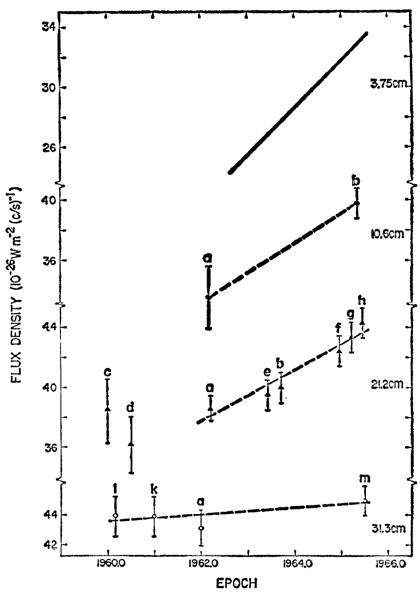
\includegraphics[scale=0.33]{oldflux-}};
					
					\begin{scope}[x={(image.south east)},y={(image.north west)}]
%						\draw [step=.02, gray,thin, opacity=0.5] (0,0) grid (1,1);
%						\draw [step=.1, black, opacity=0.5] (0,0) grid (1,1);
						
						\node[] at (0.4, 0.925) {\tiny(\citeauthor{oldflux} \citeyear{oldflux})};
						
%						horizontal
						\draw[dashed, ultra thick, line cap=round, MyOrange, opacity=0.7] (0.145, 0.3) -- (0.5, 0.3);
						\draw[dashed, ultra thick, line cap=round, MyOrange, opacity=0.7] (0.145, 0.44) -- (0.86, 0.44);
%						vertical
						\draw[dashed, ultra thick, line cap=round, opacity=0.75, MyBlue] (0.5, 0.066) -- (0.5, 0.3);
						\draw[dashed, ultra thick, line cap=round, opacity=0.75, MyBlue] (0.86, 0.066) -- (0.86, 0.44);
						
						\node[MyOrange] at (0.375, 0.41) {\small\( \Delta F \approx 6 \unit{\FU}\)};
						\node[MyBlue] at (0.675, 0.2) {\small\( \Delta t \approx 3 \unit{\year}\)};
					\end{scope}
				\end{tikzpicture}
			\end{column}
			\begin{column}{0.6\textwidth}
				\only<2-3>{\begin{quotebox}
					\blockcquote{rees}{Because the {\color{MyBlue}observed intensity} of a source, for a given {\color{MyRed}surface brightness}, is proportional to the {\color{MyOrange}apparent size}}
				\end{quotebox}
				\( {\color{MyBlue}F} = {\color{MyRed}B}{\color{MyOrange}\sphericalangle} \propto 2\tfrac{\gamma vt}{R}\quad \uncover<3>{\dv{\color{MyBlue}F}{t} = 2\tfrac{\gamma v}{R} \propto \gamma} \)
				
				\uncover<3>{\begin{quotebox}
						\blockcquote{rees}{it is already clear that an expanding  source could exhibit a rate of increase of flux density high enough to explain the observations.}
					\end{quotebox}}}
				
				\only<4>{\begin{quotebox}
					\blockcquote{rees}{If, however, a source at the distance of 3C 273 were to start to explode with a velocity corresponding to \( \gamma = 5 \), and if \( H \) (measured in a frame sharing the mean particle motion) \( \sim 10^{-2} \unit{gauss} \), the flux density would have risen to\\ \( \sim 15 \unit{\FU} \) in 3 years}
				\end{quotebox}}
			\end{column}
		\end{columns}
	\end{frame}
	
	
	\begin{frame}{Konsequenz}
		\begin{tikzpicture}[every node/.style={scale=0.9}, scale=1.4]
	%		\node[inner sep=0pt] (russell) at (0,0.05){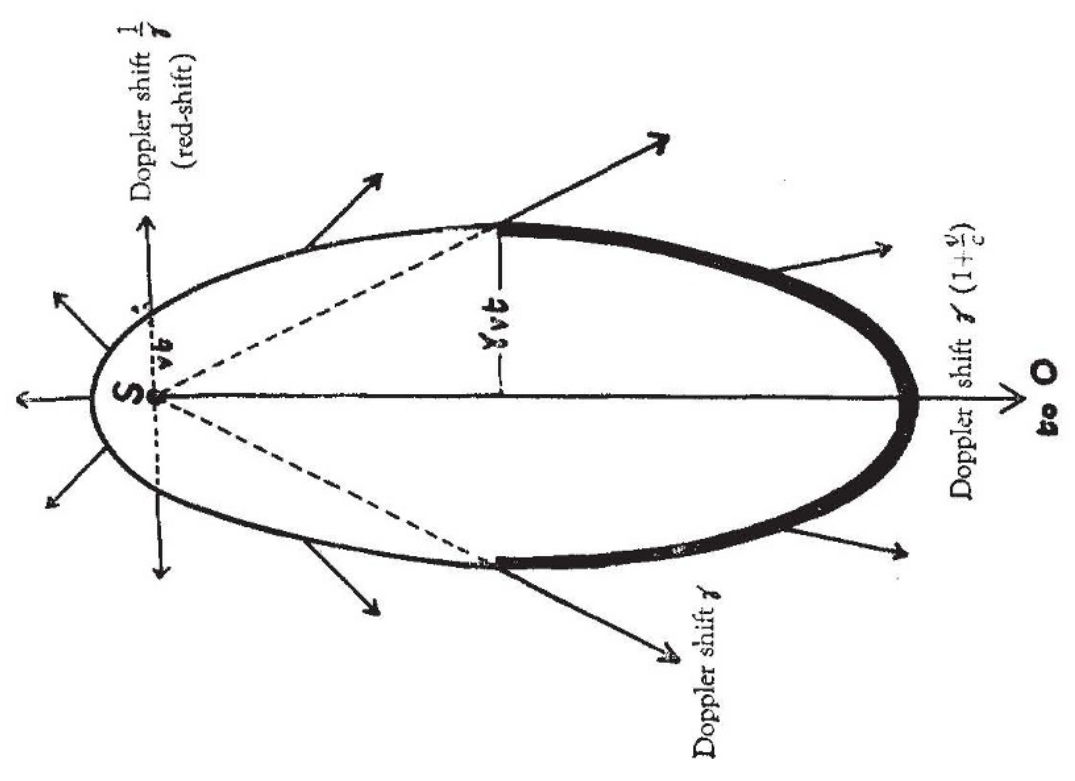
\includegraphics[scale=0.25]{bilder/aberration2}};
	
	%		\draw [step=.1, gray,thin, opacity=0.5] (-4,-2) grid (4,2);
	%		\draw [step=1, black, opacity=0.5] (-4,-2) grid (4,2);
			
			\coordinate (S) at (-2.5, 0);
			
			\draw[-latex] (S) -- (-3.5, 0);
			
			\draw[-latex] (S) -- (-3.2, 0.7);
			\draw[-latex] (S) -- (-3.2, -0.7);
			
			\draw[-latex] (S) -- (-2.5, 1.2);
			\draw[-latex] (S) -- (-2.5, -1.2);
			
			\draw[-latex] (S) -- (-1, 1.5);
			\draw[-latex] (S) -- (-1, -1.5);
			
			\draw[-latex] (S) -- (0.9, 1.7);
			\draw[-latex] (S) -- (0.9, -1.7);
			
			\draw[-latex] (S) -- (2.4, 1);
			\draw[-latex] (S) -- (2.4, -1);
			
			
			\draw[fill=bg] (-0.25,0) ellipse (2.7 and 1.1);
			
			\draw[MyBlue, line cap=round, thick] (S) -- (-2.5, 0.6) node [right, pos=0.55] {\( v t \)};
			\draw[MyRed, thick] (-0.25, 0) -- (-0.25, 1.1) node [left, pos=0.5] {\( \gamma v t \)};
			
			\draw[thick] (-0.25,0) ellipse (2.7 and 1.1);
			
			\draw[line width=2.5, MyOrange, opacity=0.75, line cap=round] (-0.25,0) [partial ellipse=-90:90:2.7 and 1.1];
			
			\draw[fill] (S) circle (0.05cm) node [below, yshift=-1] {\( S \)};
			
			\draw[-latex, semithick] (S) -- (3.5, 0) node [above left, pos=0.975] {to \( O \)};
			
%			\node[rectangle, rounded corners, draw=MyRed, align=left] at (3.5, 2.5) 
%			{\(\gamma = \frac{1}{\sqrt{1-\beta^2}}\)\\[1ex] \(\beta = \frac{v}{c} \)};
		\end{tikzpicture}
		\( \beta = \frac{v}{c} \in [0; 1] \)\\
		\( \gamma = \frac{1}{\sqrt{1 - \beta^2}} \in [1, \infty) \)
		\(\quad\Rightarrow\quad \gamma v > c \) möglich!
	\end{frame}
	
	\begin{frame}{Kosmische Jets}
		\begin{columns}
			\hspace*{-0.5cm}
			\begin{column}{0.61\textwidth}
				\vspace*{0.2cm}
				\begin{tikzpicture}
					\node[anchor=south west,inner sep=0] (image) at (0,0) {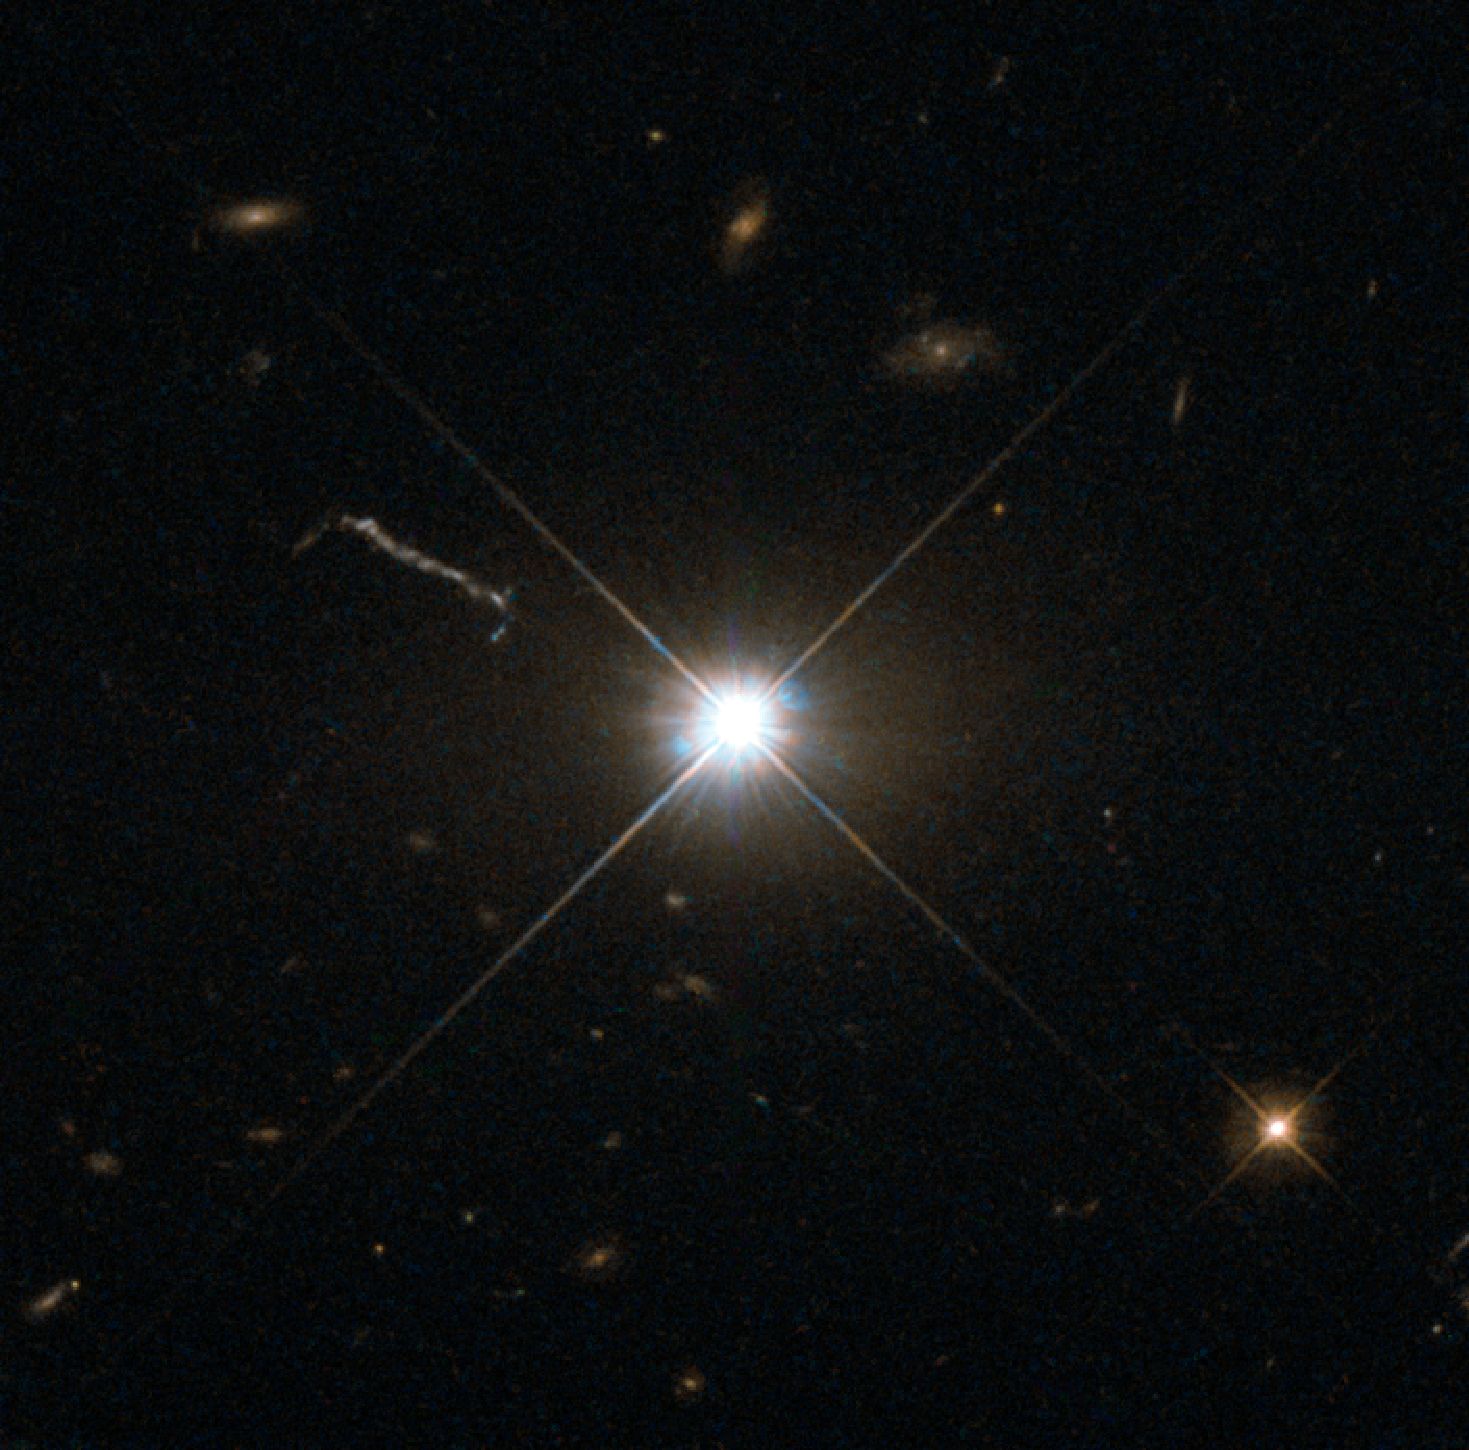
\includegraphics[scale=0.3]{3c273new}};
					
					\begin{scope}[x={(image.south east)},y={(image.north west)}]
						\node[] at (0.2, -0.02) {\tiny 3C 273 © ESA/HUBBLE \& NASA};
					\end{scope}
				\end{tikzpicture}
			\end{column}
			\begin{column}{0.375\textwidth}
				\begin{tikzpicture}
					\node[anchor=south west,inner sep=0] (image) at (0,0) {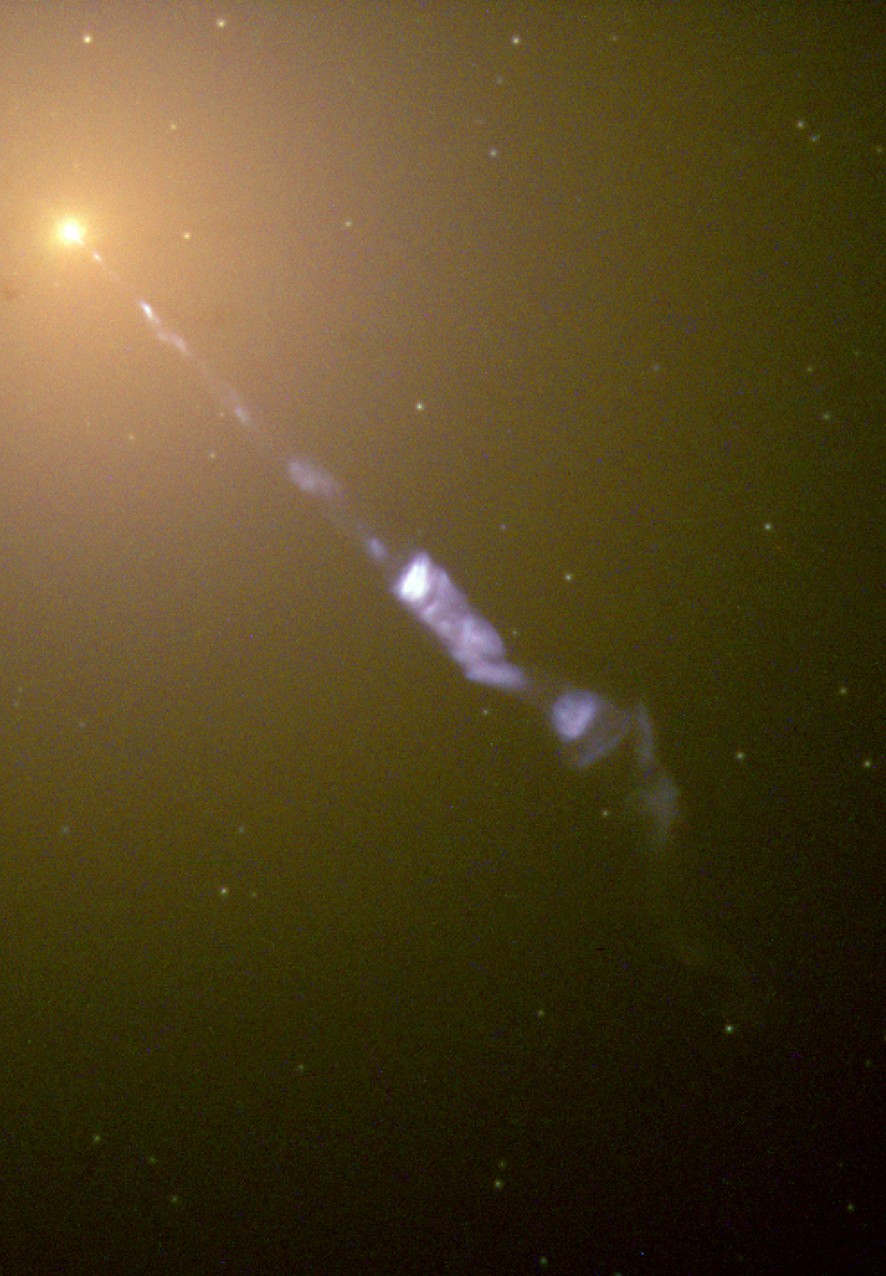
\includegraphics[scale=0.3]{M87_jet}};
					
					\begin{scope}[x={(image.south east)},y={(image.north west)}]
						\node[] at (0.3, -0.02) {\tiny M87 © ESA/HUBBLE \& NASA};
					\end{scope}
				\end{tikzpicture}
			\end{column}
		\end{columns}
	\end{frame}
	
%% 	######### Recap #########
	\begin{frame}{Recap}
		\hspace*{-1cm}
		\begin{tikzpicture}[xscale=5, yscale=2.5]
			\node (A) at (0, 0) {%Axis Angles
				\tdplotsetmaincoords{70}{90}
				%Macros
				\pgfmathsetmacro{\rvec}{6}
				\pgfmathsetmacro{\thetavec}{65}
				\pgfmathsetmacro{\phivec}{55}
				
				\pgfmathsetmacro{\dphivec}{30}
				\pgfmathsetmacro{\dthetavec}{20}
				%Layers
				\pgfdeclarelayer{background}
				
				\pgfsetlayers{background, main}
				\begin{tikzpicture}[tdplot_main_coords, scale=0.2]
					%Coordinates
					\coordinate (O) at (0,0,0);
					%
					\tdplotsetcoord{A}{\rvec}{\thetavec}{\phivec}
					\tdplotsetcoord{B}{\rvec}{\thetavec + \dthetavec}{\phivec}
					\tdplotsetcoord{C}{\rvec}{\thetavec + \dthetavec}{\phivec + \dphivec}
					\tdplotsetcoord{D}{\rvec}{\thetavec}{\phivec + \dphivec}
					%
					\tdplotsetcoord{A'}{\rvec + 4}{\thetavec}{\phivec}
					\tdplotsetcoord{B'}{\rvec + 3}{\thetavec + \dthetavec}{\phivec}
					\tdplotsetcoord{C'}{\rvec + 1}{\thetavec + \dthetavec}{\phivec + \dphivec}
					\tdplotsetcoord{D'}{\rvec + 2}{\thetavec}{\phivec + \dphivec}
					%		
					%Help Lines
					\begin{pgfonlayer}{background}
						%Up
						\draw[] (O) -- (A');
						\draw (O) -- (B');
						\draw (O) -- (C');
						\draw[] (O) -- (D');
					\end{pgfonlayer}
					
					\begin{scope}
						%Fill Color
						\begin{pgfonlayer}{main}
							\clip[canvas is zy plane at x=0] (\rvec - 0.09,0) arc (0:200:\rvec - 0.09);
							%Front
							\filldraw[opacity=0.6, color=black, fill=MyOrange, thick] (A) to[bend left=4] (B)  to[bend left=2] (C) to[bend right=6.5] (D) to[bend right=4] cycle;
						\end{pgfonlayer}
						
						\draw[canvas is zy plane at x=0, ultra thick, MyBlue] (\rvec - 0.1,0) arc (0:200:\rvec - 0.1);	
					\end{scope}
			\end{tikzpicture}};
			
			\node (B) at (1, 0) {\begin{tikzpicture}[scale=0.4, every node/.style={scale=2}]
					\begin{axis}[
					axis lines = left,
					axis line style = ultra thick,
					xlabel = \(t\) in Jahren,
					ylabel = {Fluss},
					enlargelimits=true,
					xtick=\empty,
					ytick=\empty,
					xmin=0,
					xmax=6,
					ymin=1,
					ymax=2,
					tick align=inside,
					tickwidth=5pt]
					\addplot [domain=-1:0, color=MyBlue, ultra thick] {1};
					\addplot [domain=0:2, color=MyBlue, ultra thick] {x/2+1};
					\addplot [domain=2:3, color=MyBlue, ultra thick] {2};
					\addplot [domain=3:5, color=MyBlue, ultra thick] {-x/2+3.5};
					\addplot [domain=5:6, color=MyBlue, ultra thick] {1};
			\end{axis}
			\end{tikzpicture}};
			
			\uncover<2->{\node[MyRed] (C) at (1.9, 0) {\fontsize{40pt}{10pt}\selectfont\faBolt};}
			
			\uncover<4->{\node (E) at (0.45, -1) {\begin{tikzpicture}[every node/.style={scale=0.9}, scale=0.7]
					\coordinate (S) at (-2.5, 0);
					
					\draw[-latex] (S) -- (-3.5, 0);
					
					\draw[-latex] (S) -- (-3.2, 0.7);
					\draw[-latex] (S) -- (-3.2, -0.7);
					
					\draw[-latex] (S) -- (-2.5, 1.2);
					\draw[-latex] (S) -- (-2.5, -1.2);
					
					\draw[-latex] (S) -- (-1, 1.5);
					\draw[-latex] (S) -- (-1, -1.5);
					
					\draw[-latex] (S) -- (0.9, 1.7);
					\draw[-latex] (S) -- (0.9, -1.7);
					
					\draw[-latex] (S) -- (2.4, 1);
					\draw[-latex] (S) -- (2.4, -1);
					
					
					\draw[fill=bg] (-0.25,0) ellipse (2.7 and 1.1);
					
					\draw[thick] (-0.25,0) ellipse (2.7 and 1.1);
					
					\draw[line width=2.5, MyOrange, opacity=0.75, line cap=round] (-0.25,0) [partial ellipse=-90:90:2.7 and 1.1];
					
					\draw[fill] (S) circle (0.05cm);
					
					\draw[-latex, semithick] (S) -- (3.5, 0);
			\end{tikzpicture}};}
		
			\uncover<3->{\node (F) at (1.5, -1) {\begin{tikzpicture}[every node/.style={scale=0.9}, scale=0.7]				
					\coordinate (S) at (-2.5, 0);
					
					\draw[-latex] (S) -- (-3.5, 0);
					
					\draw[-latex] (S) -- (-2.5+0.7,  0.7);
					\draw[-latex] (S) -- (-2.5+0.7, -0.7);
					
					\draw[-latex] (S) -- (-2.5-0.7,  0.7);
					\draw[-latex] (S) -- (-2.5-0.7, -0.7);
					
					\draw[-latex] (S) -- (-2.5, 1);
					\draw[-latex] (S) -- (-2.5, -1);
					
					
					\draw[fill=bg] (S) circle (0.6);
					
%					\draw[MyBlue, line cap=round, thick] (S) -- (-2.5, 0.6) node [right, pos=0.55] {\( v t \)};
					
					\draw[thick] (S) circle (0.6);
					
					\draw[line width=2.5, MyOrange, opacity=0.75, line cap=round] (-2.5, -0.6) arc (-90:90:0.6);
					
					\draw[fill] (S) circle (0.05cm);
					
					\draw[-latex, semithick] (S) -- (-1.5, 0);
			\end{tikzpicture}};}
		
			\uncover<5->{\node[MyGreen] (G) at (0.15, -2) {\fontsize{40pt}{10pt}\faCheck};}
			
			\uncover<6->{\node[draw=MyOrange, rectangle, rounded corners, fill=orange!15, thick] (H) at (1, -2) {\Huge\( \gamma v > c \)};
			\node at (1.5, -2) {\fontsize{40pt}{10pt}\selectfont!!!};}
			
			\node at (0.5, 0) {\Huge\faPlus};
			\uncover<2->{\node at (1.5, 0) {\Huge\faEquals};}	
			
			\uncover<3->{\draw[-latex, thick, dashed, shorten <= 0.15cm, shorten >= 0.15cm] (C.south) to [out=-90,in=0] (F.east);}
			\uncover<4->{\draw[-latex, thick, dashed, shorten >=0.15cm, shorten <= 0.15cm] (F) -- (E) node [above, pos=0.5] {\( c =  \)const.};}
			\uncover<5->{\draw[-latex, thick, dashed, shorten <= 0.15cm, shorten >= -0.15cm] (E.west) to [out=220,in=125] (G.north west);}
			
			\uncover<6->{\draw[-latex, thick, dashed, shorten <= 0.15cm, shorten >= 0.15cm] (E.west) to [out=220,in=150] (H.north west);}
		\end{tikzpicture}
	\end{frame}
\begin{frame}[standout]
	\Huge Fragen?
\end{frame}

\appendix

\def\cbeta{0.835}
\def\time{6}
\def\Rinit{0.5}

\begin{frame}{Relativistische Expansion}
	\begin{tikzpicture}[every node/.style={scale=0.9}, scale=1.2]	
		\clip[] (-1, -3) rectangle (85, 3);
		
%		\draw [step=.1, gray,thin, opacity=0.5] (-4,-2) grid (4,2);
%		\draw [step=1, black, opacity=0.5] (-4,-2) grid (4,2);
		
		\coordinate (O) at (0, 0);
		\draw[] (O) circle (0.05) node [below, yshift=-1] {\( S \)};
		
		\node[rectangle, rounded corners, draw=MyRed] at (6.5, 2.5) {\( \beta = \cbeta,\ \gamma = 1.82 \)};
		
		\foreach \j [count=\i] in {0, 0.25, 0.59, 1.5, 2.5, 4, 5.5, 6}{
			\uncover<\i>{
				\def\time{\j}
				\node[draw=MyRed, rectangle, rounded corners, align=left, text width=1.25cm] at (7.2, 2) {\( t = \time \)};
				
				\draw[dashed] (0, 0) circle (\Rinit + \cbeta*\time);
				\draw[snake arrow, MyBlue] (-\Rinit + \j - 0.5, 0) -- (-\Rinit + \j, 0);
			}
		}
		
		\draw[fill] (-\Rinit, 0) circle (0.05);
		\only<1>{\draw[fill, MyOrange] (-\Rinit, 0) circle (0.05);}
		
		\only<2>{
				\draw[fill, MyOrange] (-0.25,  0.65) circle (0.05);
				\draw[fill, MyOrange] (-0.25, -0.65) circle (0.05);}
		\uncover<3->{
				\draw[fill] (-0.25,  0.65) circle (0.05);
				\draw[fill] (-0.25, -0.65) circle (0.05);}
				
		\only<3>{
				\draw[fill, MyOrange] (0,  1) circle (0.05);
				\draw[fill, MyOrange] (0, -1) circle (0.05);}
		\uncover<4->{
				\draw[fill] (0,  1) circle (0.05);
				\draw[fill] (0, -1) circle (0.05);}
				
		\only<4>{
			\draw[fill, MyOrange] (1,  1.45) circle (0.05);
			\draw[fill, MyOrange] (1, -1.45) circle (0.05);}
		\uncover<5->{
			\draw[fill] (1,  1.45) circle (0.05);
			\draw[fill] (1, -1.45) circle (0.05);}
		
		\only<5>{
			\draw[fill, MyOrange] (2,  1.6) circle (0.05);
			\draw[fill, MyOrange] (2, -1.6) circle (0.05);}
		\uncover<6->{
			\draw[fill] (2,  1.6) circle (0.05);
			\draw[fill] (2, -1.6) circle (0.05);}
			
		\only<6>{
			\draw[fill, MyOrange] (3.5,  1.6) circle (0.05);
			\draw[fill, MyOrange] (3.5, -1.6) circle (0.05);}
		\uncover<7->{
			\draw[fill] (3.5,  1.6) circle (0.05);
			\draw[fill] (3.5, -1.6) circle (0.05);}
			
		\only<7>{
			\draw[fill, MyOrange] (5,  1) circle (0.05);
			\draw[fill, MyOrange] (5, -1) circle (0.05);}
		\uncover<8->{
			\draw[fill] (5,  1) circle (0.05);
			\draw[fill] (5, -1) circle (0.05);}
		
		\only<8>{\draw[fill, MyOrange] (5.5, 0) circle (0.05);}
		\uncover<9->{\draw[fill] (5.5, 0) circle (0.05);
					\node[draw=MyRed, rectangle, rounded corners, text width=1.25cm, align=left] at (7.2, 2) {\( t > 6 \)};
					\draw[snake arrow, MyBlue] (-\Rinit + 7 - 0.5, 0) -- (-\Rinit + 7, 0);}
		
		\draw[-latex] (6.5, 0) -- (7.5, 0) node [above left] {to \( O \)};
	\end{tikzpicture}
\end{frame}

\begin{frame}[allowframebreaks]{Sources}
	\printbibliography
\end{frame}

\end{document}